\documentclass[preprint,journal]{vgtc}       % preprint (journal style)

%% Uncomment one of the lines above depending on where your paper is
%% in the conference process. ``review'' and ``widereview'' are for review
%% submission, ``preprint'' is for pre-publication, and the final version
%% doesn't use a specific qualifier. Further, ``electronic'' includes
%% hyperreferences for more convenient online viewing.

%% Please use one of the ``review'' options in combination with the
%% assigned online id (see below) ONLY if your paper uses a double blind
%% review process. Some conferences, like IEEE Vis and InfoVis, have NOT
%% in the past.

%% Please note that the use of figures other than the optional teaser is not permitted on the first page
%% of the journal version.  Figures should begin on the second page and be
%% in CMYK or Grey scale format, otherwise, colour shifting may occur
%% during the printing process.  Papers submitted with figures other than the optional teaser on the
%% first page will be refused.

%% These three lines bring in essential packages: ``mathptmx'' for Type 1
%% typefaces, ``graphicx'' for inclusion of EPS figures. and ``times''
%% for proper handling of the times font family.

\usepackage{mathptmx}
\usepackage{graphicx}
\usepackage{times}
\usepackage{color}
\usepackage{bm}
\usepackage{amsmath}
\usepackage{siunitx}
\usepackage{float}


%% We encourage the use of mathptmx for consistent usage of times font
%% throughout the proceedings. However, if you encounter conflicts
%% with other math-related packages, you may want to disable it.

%% allow for this line if you want the electronic option to work properly
\vgtcinsertpkg

%% Paper title.

\title{Muscular fascicle arrangement based on Laplacian vector fields}

%% This is how authors are specified in the journal style

%% indicate IEEE Member or Student Member in form indicated below
\author{Jan Kusterer, Niven Ratnamaheson, Raimund Rolfs, and Tobias Walter}
\authorfooter{
%% insert punctuation at end of each item

}

%other entries to be set up for journal
%\shortauthortitle{Schmid \MakeLowercase{\textit{et\,al.}}: ProjINF for fun and profit}

%% Abstract section.
\abstract{
	In this paper we discuss a way to implement a pipeline that allows the calculation of muscular fascicles based on the surface CT-scan of the muscle. 
	Choi and Blemker showed in advance, that simple skeletal muscles have a fascicle arrangement, which can be computed with a Laplacian vector field. 
	An electrostatic simulation considering a dielectric volume uses the same equation. 
	In this work we use a similar approach and develope a method to calculate  a specifiable amount of fibers, using the finite element mesh generator Gmsh. 
	In addition we visualize the outcome in forms of meshes and 3D-Printing.
} % end of abstract

%% Keywords that describe your work. Will show as 'Index Terms' in journal
%% please capitalize first letter and insert punctuation after last keyword
\keywords{Muscle, Fascicle, Mesh, Laplace, Electrostatic, Streamline, Biceps.}

%% ACM Computing Classification System (CCS).
%% See <http://www.acm.org/class/1998/> for details.
%% The ``\CCScat'' command takes four arguments.

\CCScatlist{ % not used in journal version
	\CCScat{Computer Graphics}{I.3.8}{Applications}{Molecular Dynamics Visualization}
	\CCScat{Simulation and Modeling}{I.6.6}{Simulation Output Analysis}{Molecular Dynamics Visualization}
	\CCScat{Computer Graphics}{I.3.7}{Three-Dimensional Graphics and Realism}{Raytracing}
}

\graphicspath{{pics/}}

%% Uncomment below to include a teaser figure.
\teaser{
\centering
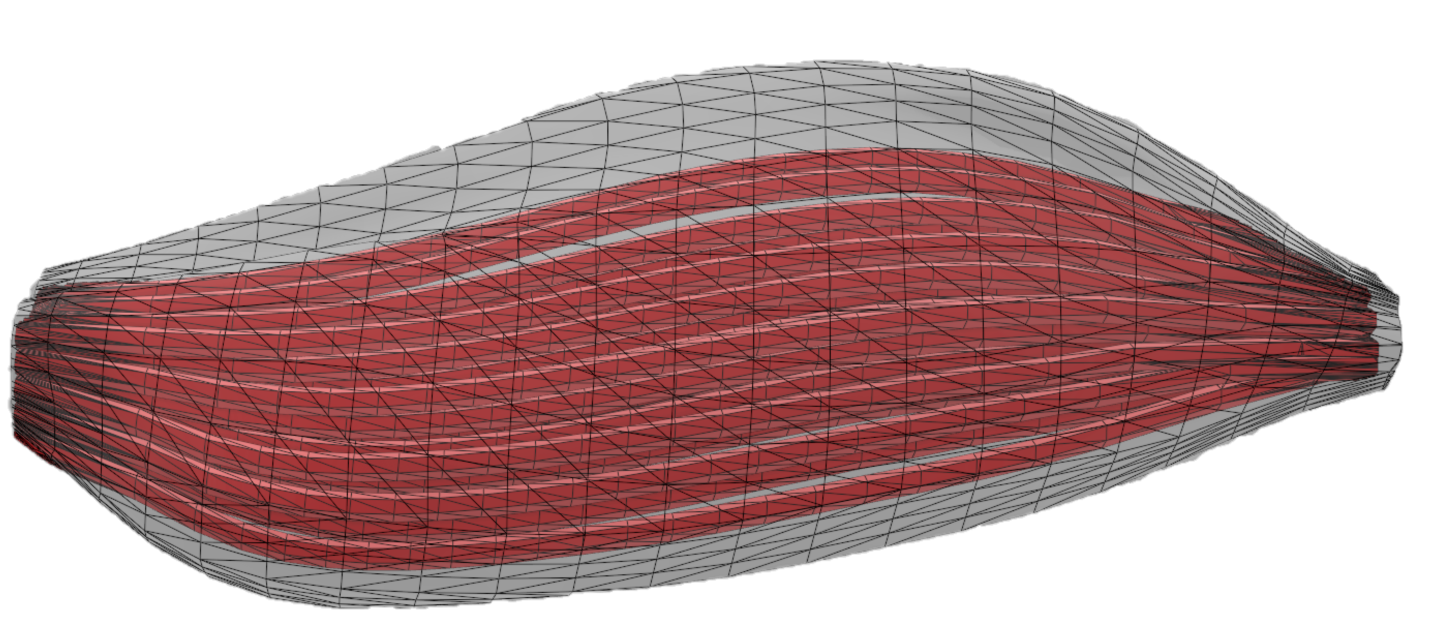
\includegraphics[width=14cm]{muscle.png}
%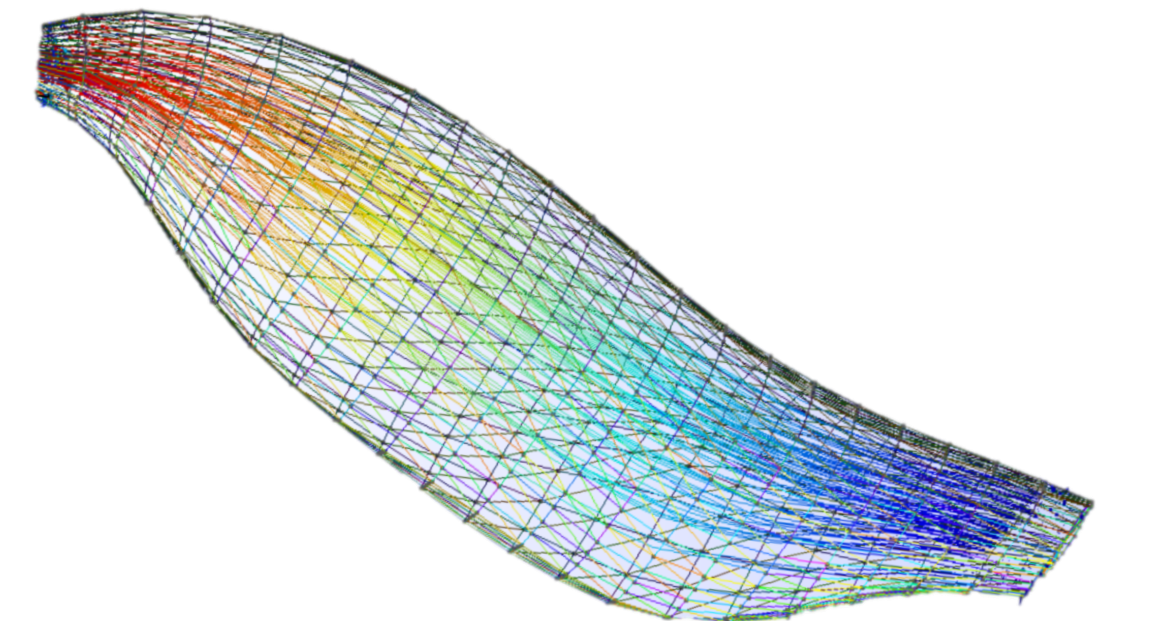
\includegraphics[width=8cm]{Muscle_with_fascicles.png}
\label{fig:teaser}
}

%%%%%%%%%%%%%%%%%%%%%%%%%%%%%%%%%%%%%%%%%%%%%%%%%%%%%%%%%%%%%%%%
%%%%%%%%%%%%%%%%%%%%%% START OF THE PAPER %%%%%%%%%%%%%%%%%%%%%%
%%%%%%%%%%%%%%%%%%%%%%%%%%%%%%%%%%%%%%%%%%%%%%%%%%%%%%%%%%%%%%%%%

\begin{document}
\maketitle
%% The ``\maketitle'' command must be the first command after the
%% ``\begin{document}'' command. It prepares and prints the title block.

%% the only exception to this rule is the \firstsection command
\section{Introduction}\label{sec:intro}
Skeletal muscles have a wide range of anatomical architectures. 
They often form a heterogeneous curvature, while the tendon and bone attachments vary in their morphology~\cite{Choi2013}. 
Each muscle consists of multiple muscle fibers which can contract via myosin motors, according to Cheng et al. 
\cite{Jiangcheng2015}, and thus create a force pulling on the bones. 
Each motor is organized as a chain of contractile parts, called sarcomeres. 
The fibers are bundled into fascicles, which contain 10 to 100 fibers and are sheathed by a tissue.
This protects and stabilizes the fibers when under load.

According to \cite{Etemadi.et.Al.} the biceps of an athletic individual has around 300.000 muscle fibers, which are single cells approximately 50 \si\micro m in diameter and several centimeters long \cite{Cooper2000}. 
Each fiber has a thick myosin filament and a thin actin filament, which surrounds the myosin. 
During the process of muscle contraction, the actin and myosin filaments slide past each other resulting in shortening of the fiber.

Since the mechanical force is transmitted along the muscle fibers, it is important for biomechanical simulations to obtain an adequate representation of their trajectories. 
In this way we can get much more realistic geometries e.g. of a contracted biceps.
However, this is not a simple task because of the complexity and diversity of the various muscles. 
To simplify the problem by a small degree, we can simulate the fascicles instead of every single fiber.

To simulate the contraction of a muscle we need an approximation of the fascicles, that stretch across the muscle. 
Although we can see them with our bare eyes, it is not easy to determine their pathway. 
There are other measurements such as the dissection of cadaver, which are limited to a few sparse locations, and ultrasound imaging, which is limited to a two-dimensional image plane.
The only three-dimensional technique to visualize the trajectories of the fascicles is diffusion tensor magnetic resonance imaging (DT-MRI) \cite{Choi2013}.
The tracing algorithm however is prone to noise in the acquired data.
Therefore, we need a method to calculate the trajectories of these fascicles in a three-dimensional space.
Muscles are often modeled using a lumped-parameter approach that assumes a simplified arrangement of fascicles. 
However, as Choi and Blemker \cite{Choi2013} stated, these models are not able to cover three-dimensional deformations.
One of the more promising approaches is using a Laplacian vector field as presented by Choi et al. \cite{Choi2013}. 

The goal of our work is the approximation of muscle fascicles based on the 3D-model of a muscle, primarily the musculus biceps brachii, with an approach using a Laplacian vector field. 

In the following sections we will first take a look into the methods. 
There we will explain our pipeline and give an outlook on the necessary steps before they are explained in detail. 
We will explain how we implemented the Laplace equation in Gmsh and describe the structure of our simulation. 
After that, the visualization and printing will be discussed and we identify some problems. 
In the end, we discuss the choices we made and talk about the resulting fascicles, as well as draw a conclusion in which we determine possible improvements and address potential future work.

%
%% \section{Introduction} %for journal use above \firstsection{..} instead
%
%\todo{Cite some stuff: bullshit~\cite{lipsa2011visualization} and simulation~\cite{hocker:084707}.}
%
\section{Methods}

To accomplish our goal, we need a tool to easily mesh the biceps and render it, while calculating an partial differential equation. 
Gmsh ~\cite{Geuzaine2009} is used for generating 3-D finite element meshes with built in pre- and post processing. 
We use it for multiple reasons as it is free software that features it's own scripting language, which uses code similar to C++ with loops, conditionals and user-defined macros.
We use these features, because they match our needs for meshing, simulation and analysis of the model. 
It can be compiled without the GUI, for use directly from the command line. 
For other manipulations and computations we use Python.

The first step when calculating streamlines is to acquire a 3-dimensional model of a muscle, in our case the biceps.
There are a couple of ways to do this.
We got our model from a computed tomography scan (CT-scan).
Although the scan was of decent quality, the mesh was incomplete due to some holes in the surface, possibly due to data noise during the CT-scan.
Repairing these holes is the first step in our pipeline (figure \ref{fig:flow}). 

The STL-file does not connect the surface triangles with its neighbors, resulting in many independent surfaces. 
Gmsh however needs one big surface to create a volume in which we can compute the streamlines. 
In order to connect all the small surfaces, we reclassify the mesh and we thus connect all the surfaces to one big hull.
This procedure is step 3 in our pipeline (figure \ref{fig:flow}). 
3D-Meshing the volume is done completely by Gmsh during the execution of our script. 

The reclassified muscle can then be reassembled within a Gmsh specific script file.
While we run this script, we also detect the inflow and outflow surfaces for later steps.
This is done by executing a python program. 
 
Since a Laplacian vector field yields reasonable results when simulating fascicle arrangement, we use a simulation of an electric field, for the reason that it implements the Laplacian equations. 
GetDP the solver, used by Gmsh, calculates the gradient inside the biceps' mesh.

The calculations result in many vectors which indicate the direction and force which apply on the  streamlines. 
On this vector-view we apply the streamlines-plugin which results in decent streamlines in the biceps brachii.
This procedure is step 2 in our computation in the flowchart.

With help of another Python script we extract the streamlines from the post-processing file and write them into a new geo file. 
Merging this file with the original biceps surface displays their arrangement, as can be seen in the title picture.
\begin{figure} 
	\begin{center}
		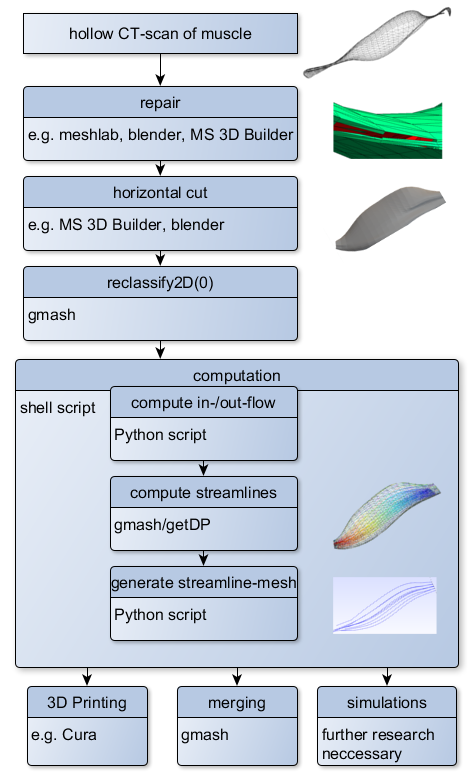
\includegraphics[width=0.79\linewidth]{flow006.png}
	\end{center}
	\caption{Flowchart of our Pipeline}
	\label{fig:flow}
	
\end{figure}
\subsection{Preparations}
As we start from a CT-scan we first need to check whether the volume is complete and closed, since noise can corrupt the data during scanning.
The biceps, as the name indicates, has two heads. 
Close to the fork, there are small holes in the surface, as seen  in figure \ref{fig:holes}, which cause Gmsh to crash, when meshing the model. 
In oder to proceed we have to check for holes and close them.
Therefore we use a repair feature which most of the common 3D modeling tools share. 

For easier computation and better outcome of the streamlines, we cut the muscle horizontal just below the fork and above the main volume (assuming that the fork is pointing upwards or rather along the z-axis). 

\begin{figure} [H]
	\begin{center}
		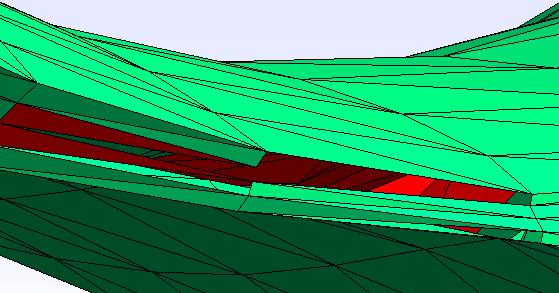
\includegraphics[width = .6\linewidth]{holes.png}
	\end{center}
	\caption{Holes in the forked area of the biceps, which need to be closed. The inside of the biceps is colored red for better contrast.}
	\label{fig:holes}
\end{figure}

\subsection{Reassembling}
The stl-file does not connect the surface triangles with its neighbors. 
Gmsh however needs one big surface to create a volume in which we can compute the streamlines. 
To connect all the small surfaces, we use the reclassify option with a threshold of 0.
This runs an edge-detection for all triangles with an angle to its neighbor greater than \ang{0}. 
This excludes the two cut surfaces, since these surfaces all have an angle of \ang{0}. 
The prepared muscle is then processed in our pipeline, see Figure ~\ref{fig:flow}. 
Finally we can recombine all the detected surfaces to one big surface. 
The recombination is done within Gmsh by iterating over the surfaces and declaring the recombined surface as one. 
The basic operations done in the script are to be seen in the code fragment below. 
From all the surfaces, a compound surface is created which then is combined in a surface loop. 
The parameters used, for example Loop(10000) means that a new loop, with the number 10000 as a name, is defined. 
In the next line, the 10000 is used again to reference the loop, which is then declared as the boundary of a volume with the number 100 as for reference. 

\begin{verbatim}
//declare ss as surface
ss[] = Surface {:};
//combine the surfaces
Compound Surface{ss[]};
//create a surface loop
Surface Loop(10000) = {ss[]};
//define the volume inside the loop
Volume(100) = {10000};
//physical entities are needed for simulation
Physical Surface (100) = {ss[]};
Physical Volume ("Body",10) = 100;
//meshing 3D when executing script
Mesh 3;
//disable Automatic Remeshing
Solver.AutoMesh = 0;
\end{verbatim}

With this new reassembled 3D-structure we now run our python script to detect the two cut surfaces.
As we said before, the length of the biceps is roughly orientated along the z-axis of the coordinate system. 
Since we cut the biceps orthogonal to the Z-axis of the model, the process is fairly simple.
We look for all vertices with the highest z-coordinate for the upper boundary and the lowest z-coordinate for the lower boundary, respectively.
These two sets are grouped and form two new surfaces. 
With this surface we save the maximum and minimum of the y- and x- coordinates for later use of the streamlines. 
We do this to cover the whole surface with the starting points of the streamlines.
Physical entities are declared as items, that are used in the simulation as they are needed for GetDP to function properly.
In this case the two surfaces identified by the python script, the volume and the surface of the muscle are our physical regions. 

\subsection{Meshing}
Meshing with Gmsh is fairly easy. 
By default Gmsh chooses between three 2D algorithms and two 3D algorithms.
The automatic algorithm selection tries to select the most appropriate for the given structure.

For 2D algorithms there are "MeshAdapt", "Delauny" and the "Frontal" algorithm.
Every one of them has different use cases. 
According to Gmsh the "MeshAdapt" works best for very complex, curved surfaces.
"Frontal" is the best choice, when high element quality is important and "Delauny" is fastest for large meshes of plane surfaces.
As stated in the manual for Gmsh the automatic selection chooses "Delauny" for plane surface and "MeshAdapt" for all other surfaces. 

For 3D algorithms there are "Delauny" and "Frontal". 
The “Delaunay” algorithm is the most robust and the fastest. 
However, this algorithm will sometimes modify the surface mesh, and is thus not suitable for producing hybrid structured/unstructured grids and in that case the “Frontal” algorithm should be preferred. 
As our mesh is unstructured, the "Delauny" is our algorithm. 
The quality of the elements produced by both algorithms is comparable.
For our 3D mesh, first the 2D surfaces and then the volume is meshed. 
In the code fragment, already shown in the "Reassembling"-chapter, the line "Mesh 3;" tells the program to do exactly this: mesh 2D first and then mesh 3D.
%\begin{figure}
%	\begin{center}
%		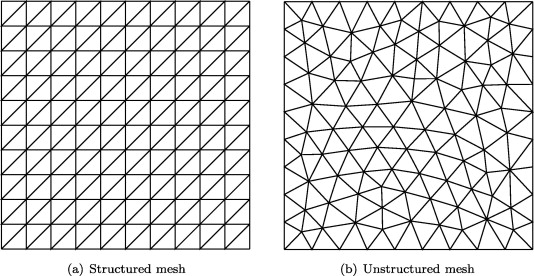
\includegraphics[width=\linewidth]{gridCompare.jpg}
%	\end{center}
%	\caption{Comparisson of structured and unstructured grids ~\cite{}}
%	
%\end{figure}
%-------------------------------------------------------------------------

\subsection{Simulation}
Gmsh's solver GetDP features a plugin, which calculates the streamlines based on the vector field. 
Therefore we need a simulation on fluid flow or similar. 
Electrostatics in a dielectric environment meets the requirement for the Laplace equation, as well as thermodynamics does.
We tried out both thermodynamic and electrostatic simulation. 
In figure ~\ref{fig:L} we see the unsatisfying results we obtained using the thermodynamic approach. 
As we compare the results of both simulations, we notice streamlines leaving the the model at the corner of the L-figure. 
The result of the electrostatic simulation is spread evenly and has fewer vortices. 
It has an overall better representation of the model.

\begin{figure}
	
	\begin{minipage}{\linewidth}
		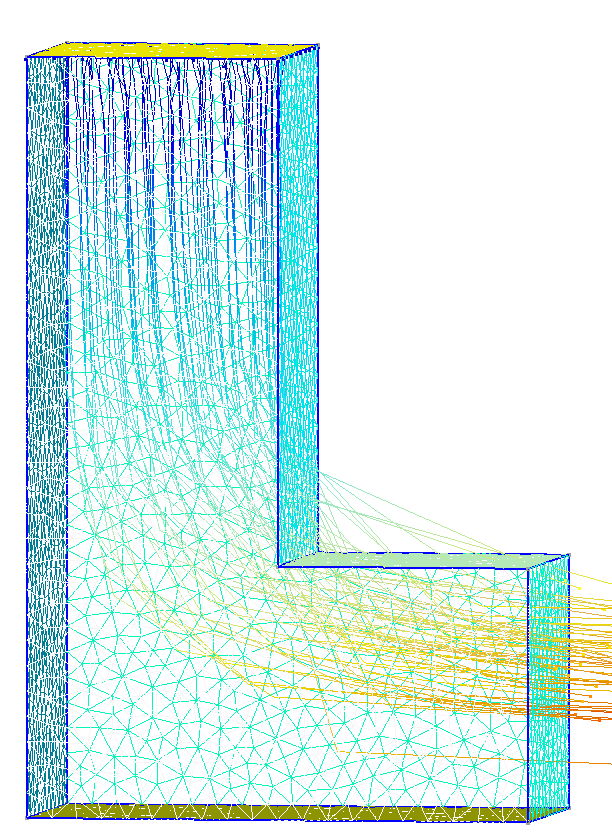
\includegraphics[width=.5\linewidth]{L.PNG} 
		\includegraphics[width=.53\linewidth]{L-ele.png}
		\caption{Comparison of thermodynamic (left) and electrostatic (right) calculation.}
		\label{fig:L}
	\end{minipage}
\end{figure}

The Laplace equation can be used in 3D just as in 2D. 
GetDP's problem definition files (.pro) are used to describe the models for simulation. 
In this model we consider the calculation of the electric field given a static distribution of electric potential. 
This matches to an "electrostatic" physical model. 
On one end of the muscle we have a conducting surface on top of a dielectric volume, called "Body".
A Dirichlet boundary condition sets the potential on the boundary of the conducting surface , called "Electrode", to 10 mV and to 0 V on the other end of the muscle, called "Ground".
A homogeneous Neumann boundary condition is defined on the surface of the muscle to truncate the domain.

We based our problem definition on the tutorial for electrostatics ~\cite{Geuzaine2009}.
The structure of the file is as follows:

\begin{description}
	\item[Group]
	Start by giving meaningful names to physical regions defined in the mesh file.
	We only use the regions body, electrode and ground. 
	After that we define abstract regions, that are used below.
	\item[Function]
	Here we define material laws.
	We choose the dielectric permittivity of our muscle to be $\epsilon = 8.854187818 *10^{-12}$, the electric constant.
	\item[Constraint]
	The Dirichlet boundary condition is defined piecewise. 
	The constraint "Dirichlet\_Ele" is invoked later in the FunctionSpace.
	\item[Group]
	This is the domain definition of the FunctionSpace, which lists all regions on which a field is defined. 
	The domain contains both the volume and the surface of the muscle.
	\item[FunctionSpace]
	The FunctionSpace is used to pick the electric scalar potential. 
	The solution is defined  by:\newline
	-the domain definition\newline
	-a type, in our case a scalar field\newline
	-a set of basis functions which are scalar nodal basis functions for the finite element method\newline 
	-a set of entities to which the basis functions are associated (here all the nodes of the domain)\newline
	-a constraint (here the Dirichlet boundary conditions)
	
	\item[Jacobian] 
	Jacobians are used for specifying the mapping of elements in the mesh.
	"Vol" represents the classical 1-to-1 mapping for identical dimension whereas "sur" represents the mapping between 2D and 3D and "lin" is used to map line segments to segments in three dimensional space.
	
	\item[Integration]
	The "Integration" segment specifies how many points are used for the Gauss quadrature rules. 
	We use 3 points for lines and 4 for triangles.
	
	\item[Formulation]
	A GetDP formulation encodes a weak formulation of the partial differential equation. i.e. 
	
	
	\[-\nabla (\varepsilon *\mathrel{grad} v) = 0\]
%	\begin{equation*}
%	\nabla (\varepsilon *grad\ v) = 0
%	\end{equation*}
	
	In our case this weak formulation involves finding v such that
	\[-\langle \nabla (\varepsilon *\mathrel{grad} v), v' \rangle _{VolEle}= 0\]
	for all functions v'. $\langle .,. \rangle _{VolEle}$ denotes the inner product over the domain "VolEle". 
	In these equations this domain is our biceps. 
	If v' is differentiable, we usually can find v by using integration by parts with Green's identity:
	\[\langle \epsilon * \mathrel{grad} v, \mathrel{grad} v' \rangle _{VolEle} + \langle n * \epsilon * \mathrel{grad} v, v' \rangle _{BndVolEle} =  0\]
	for all v', where "BndVolEle" is the boundary of "VolEle" (the surface of our biceps). 
	In this equation the surface term vanishes, since there is either no function v' or the first factor of the inner product is zero.
	Thus, in our simulation, we are looking for functions v such that 
	\[
	\langle {\epsilon * \mathrel{grad} {v}, \mathrel{grad} v'} \rangle _{VolEle} =  0
	\]
	
	holds for all v'.
	\begin{verbatim} 
	Equation {
	Integral{[epsilon[] * Dof(d,v), {d v}]; 
	In VolE le; Jacobian Vol; Integration Int
	 }
	}
	\end{verbatim}
	
	This "Integral" statement in the formulation is a representation of this weak formulation. 
	It features four by semicolons separated arguments:
	
	-the density\newline
	-the domain of integration, \newline
	-the Jacobian of the transformation, \newline
	-the integration method to be used.
	
	\item[Resolution]
	In the resolution it is specified what to do with the weak formulation. 
	We simply generate a linear system, solve it and save the solution.  
	\item[Post Processing]
	There are two parts of post-processing available in GetDP. 
	First we can evaluate the outcome of the formulation. 
	Here the quantities are the scalar electric potential, the electric field and the electric displacement.
	The second part are post-processing operations. 
	In our case the streamline generation is done here. 
	Here the script, which detects the inflow and outflow surfaces, writes the X/Y/Z values so that we get a good coverage of starting points for our streamlines. 
	The operation is then run and the output saved to a post-processing file (.pos).
	\end{description}

\begin{figure}
	\begin{center}
		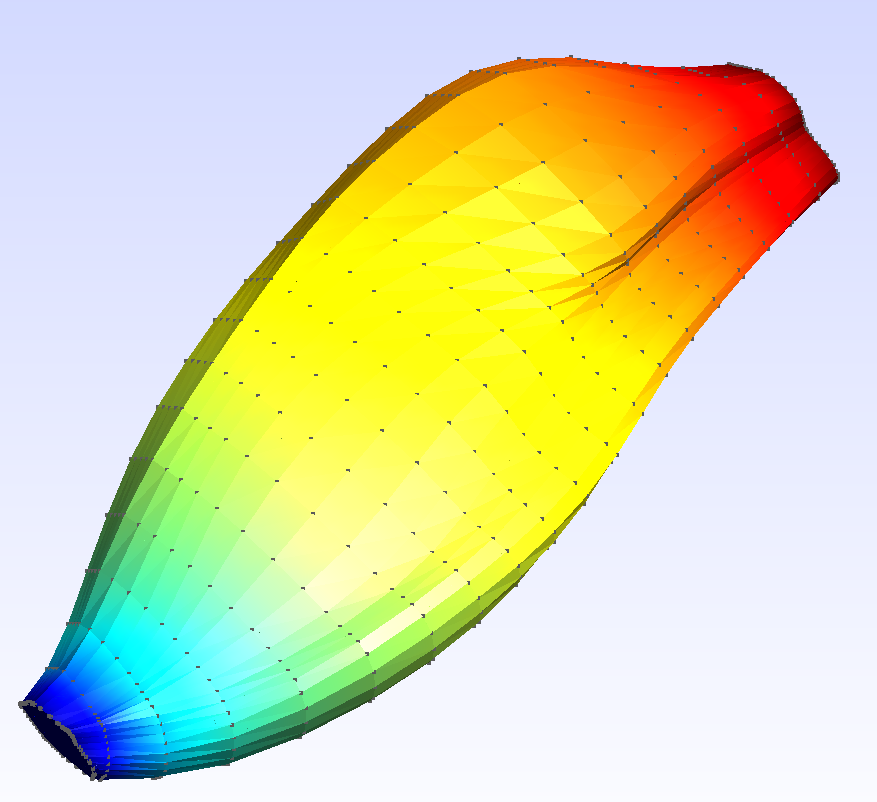
\includegraphics[width=.7\linewidth]{Sim.png}
	\end{center}
	\caption{The cut biceps after the simulation. The colors show the distance from the inflow based on the vector field.}
	\label{fig:sim}
\end{figure}

\subsection{Streamlines}
We now use the earlier mentioned plugin within the post processing described above, which calculates streamlines. 
The starting points of the streamlines are on the upper surface of the biceps, which was calculated in the reassembling section. 
The number of streamlines can be set when executing the pipeline.
The parameters are given as number of points on the X- and Y- axis. 
The extents of the surface, are the minimal and maximal X and Y values. 
That is why not all of the streamlines will start inside of the muscle. 

Additionally, we can set the number of steps we want to execute  and the length of a step.
The length of the vectors for the streamlines depend on the potential at the point of calculation at that timestep.
Afterwards, instead of extracting the complete streamlines, the exported file only contains the starting point and vectors to each point of the streamlines. 
This file consists an entry for the number of timesteps or points respectively, followed by the x-, y- and z-displacement from the starting point to each individual point of the streamline.
This however can't be imported into Gmsh since it will only display these vectors and thus we process this data. 

\section{Representation of Data}
Our next step is to sum up the vectors of each streamline separately. 
This is done by our python script streamline-converter, which gets the vector data from the muscleStreamline.pos file. 
Furthermore, the script creates a new file streamlines.geo with the data of each streamline in it. 
All in all, we can now use Gmsh to merge the streamlines.geo file with our biceps surface to visualize the result. 
However there are multiple ways to represent the streamlines. 
Another way to visualize the result is 3D-printing the streamlines.

\subsection{Printing}
Currently the streamlines are lines without any volume, but to print them they need to be thickened. 
In order to print the fascicles, a python script needs to be executed, which creates points along the streamlines at the target radius, resulting in a tube.
These points are then connected and meshed. 
We chose the profile of the tubes to be hexagonal.

After a volume is created, all of the streamlines are combined into one stl file. 
Streamlines that start outside of the biceps will get erased in this step, because they will not have any points in the file. 
In order to simplify the model, we reduced the amount of fascicles to a reasonable number of 49, which still allowed to illustrate the generated streamlines.

The 3D-Printer we use is the \textit{Ultimaker 3 extended}, which is equipped with two extruders (figure \ref{fig:3dPrinter}). 

\begin{figure}
	\centering
	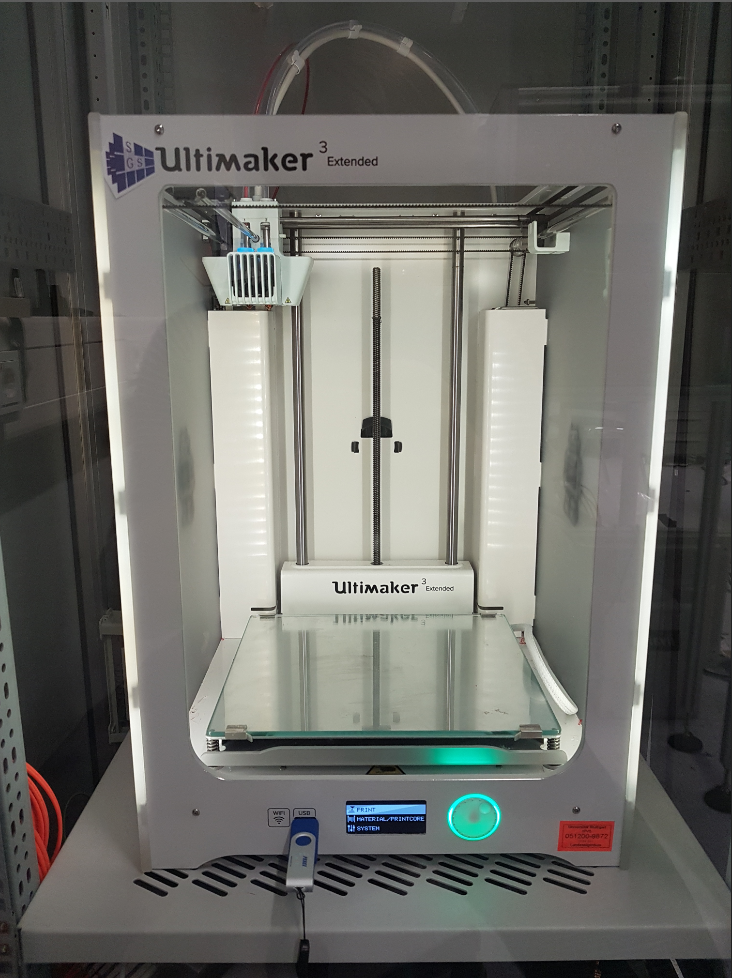
\includegraphics[width=.75\linewidth]{ultimaker-pinter2.png}
	\caption{The Ultimaker 3 extended}
	\label{fig:3dPrinter}
\end{figure}

The software used to slice and prepare the print is Cura. 
Our first approach was to subtract the muscle fibers from the full biceps volume using blender in order to have a hollowed out model with space for the fibers. 
This gives us the option to print with two different materials or colors e.g. transparent muscle and red fascicles inside as shown in \ref{fig:printedBiceps}. 

We tried several ways of printing with a clear material but we didn't get a reasonable printed sample which had a visible interior, because the filament was not as transparent as we expected it to be.
Our second approach involved cutting the biceps into two separate halves in which we are able to insert the red fascicles. 
This print however failed because the nozzle of the printcore responsible for the support got clogged. 

Our final solution (figure \ref{fig:printedBiceps}) was to print the whole model of the muscle without the fascicles and to cut it in two halves after finishing printing.  
We also tried cutting the fascicles in two halves and printing them separately, which resulted in a more stable print. 
Then, we simply glued these halves together.
The only prints which were somehow suitable to visualize our results were some test-prints as seen in figure \ref{fig:printedBiceps}.

\begin{figure}[H]
		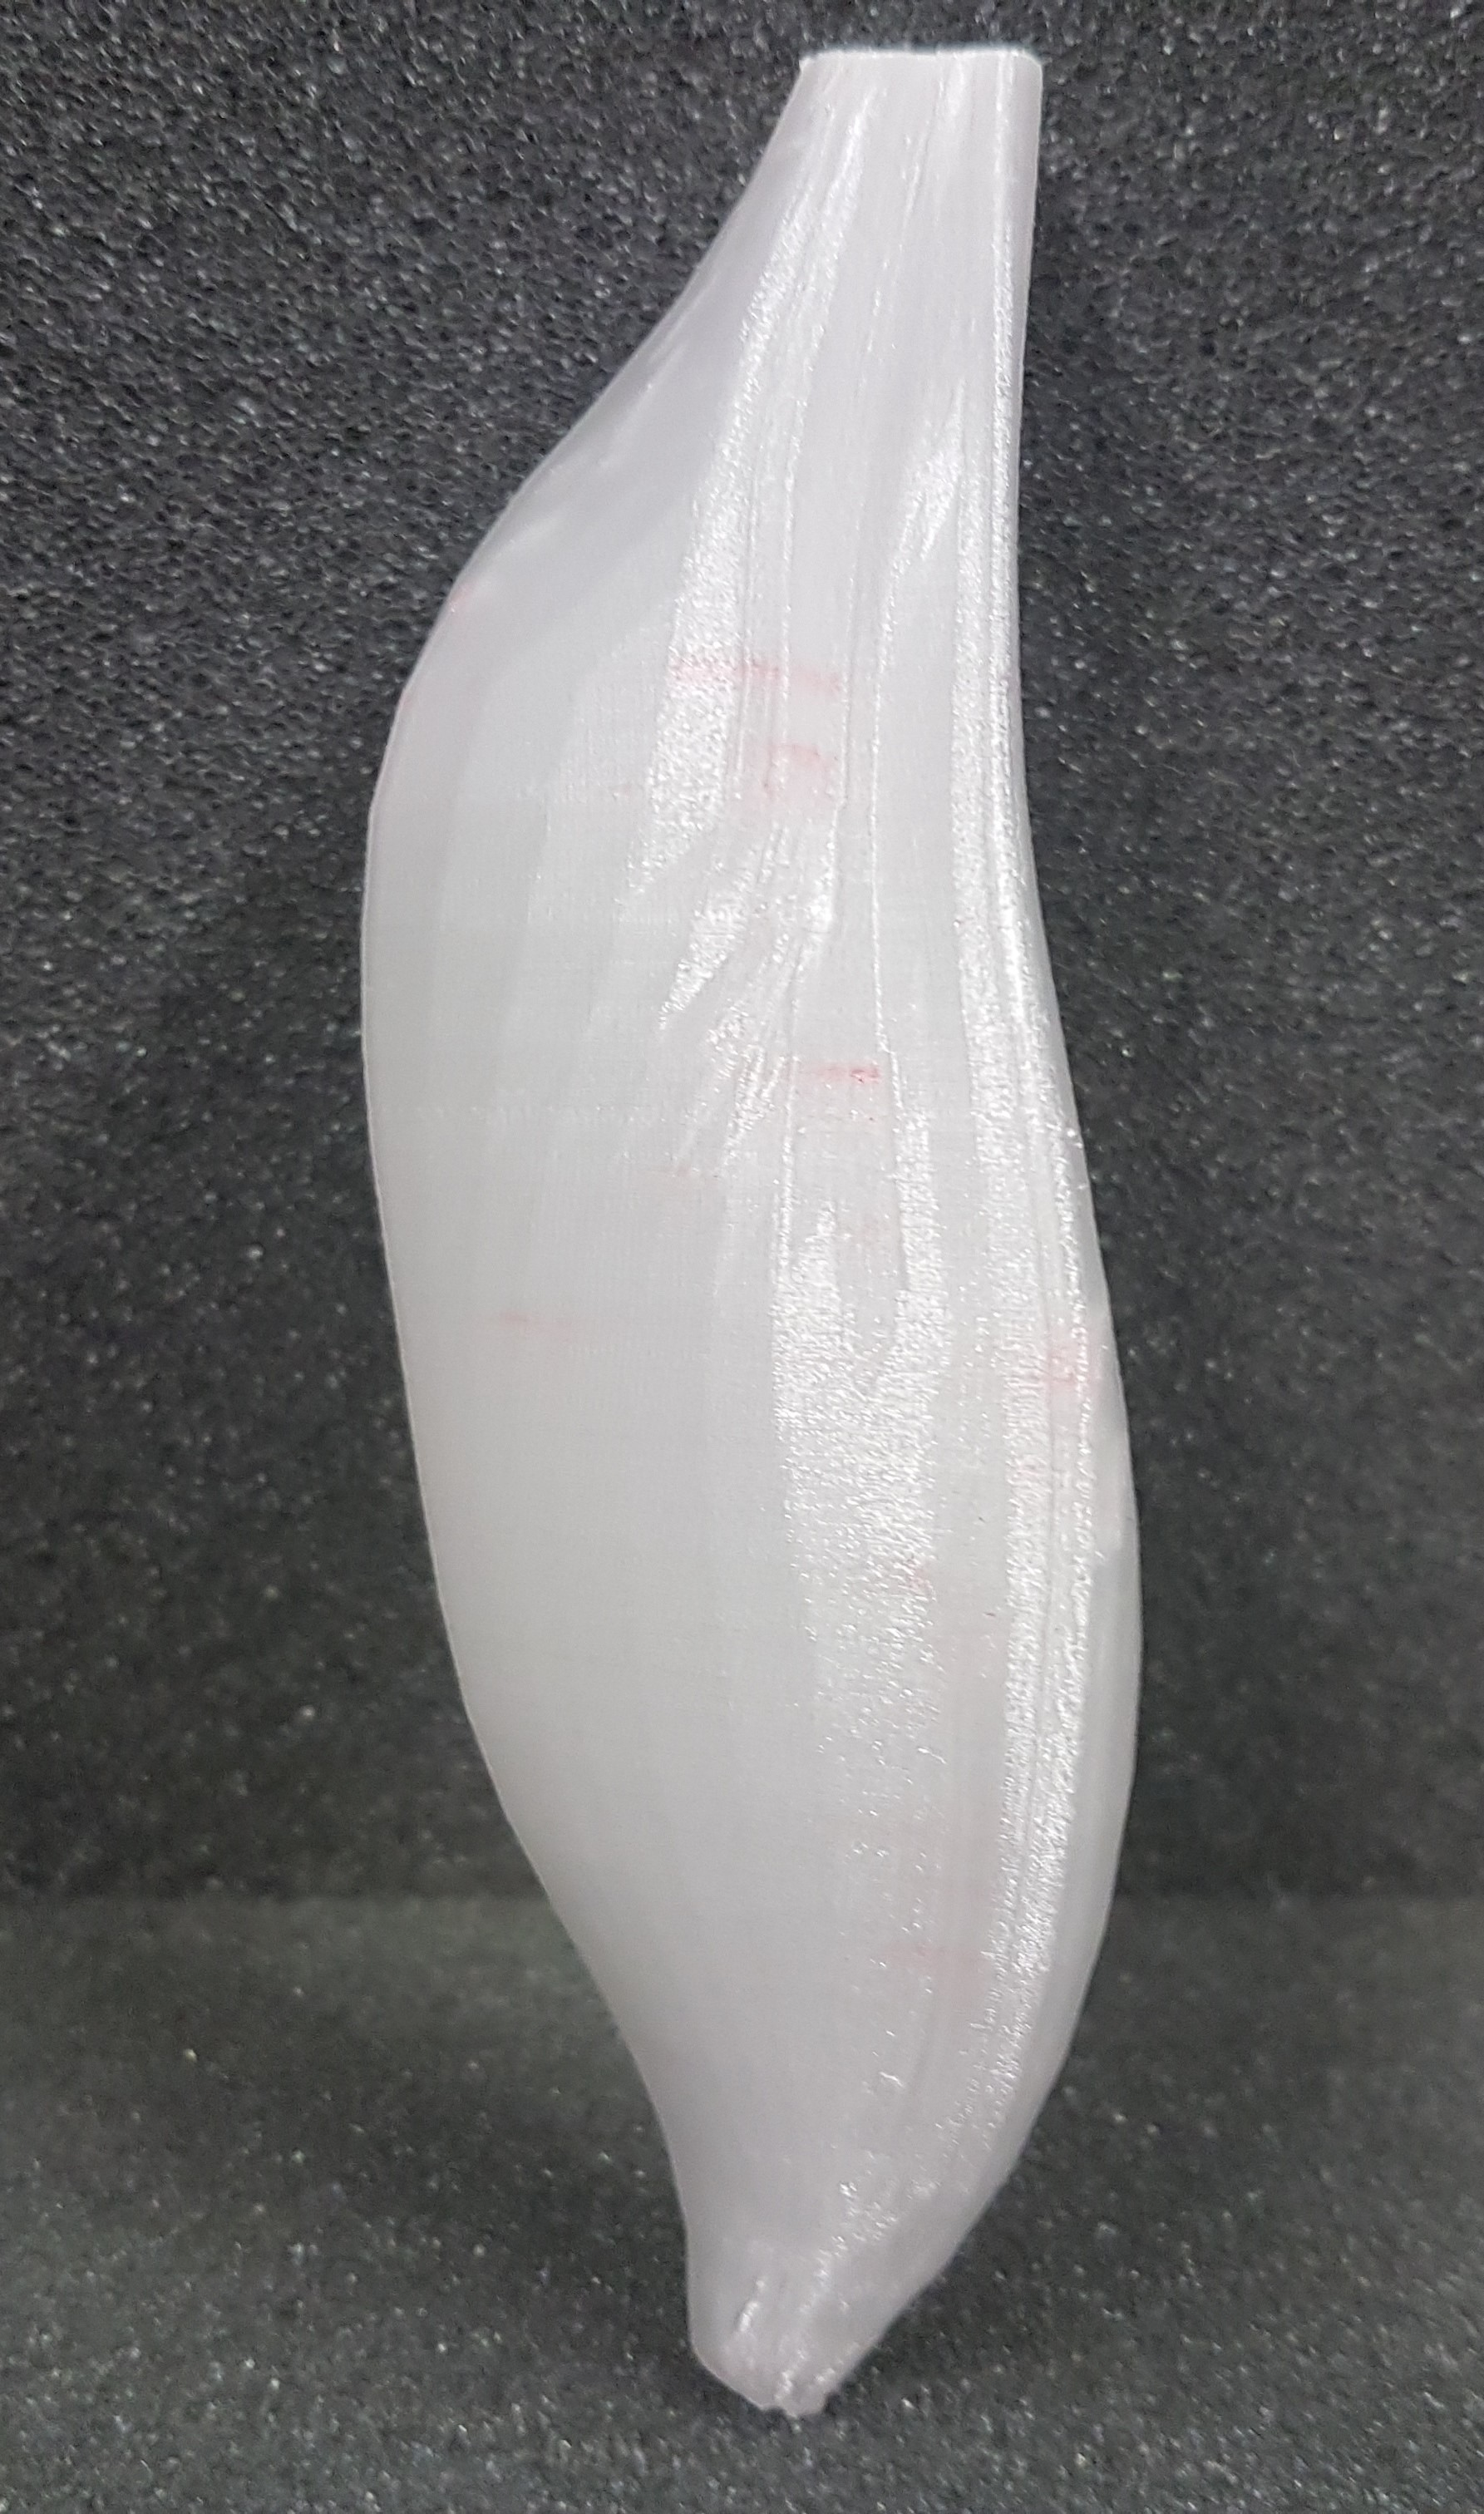
\includegraphics[width=.5\linewidth]{muscle_print.jpg} 
		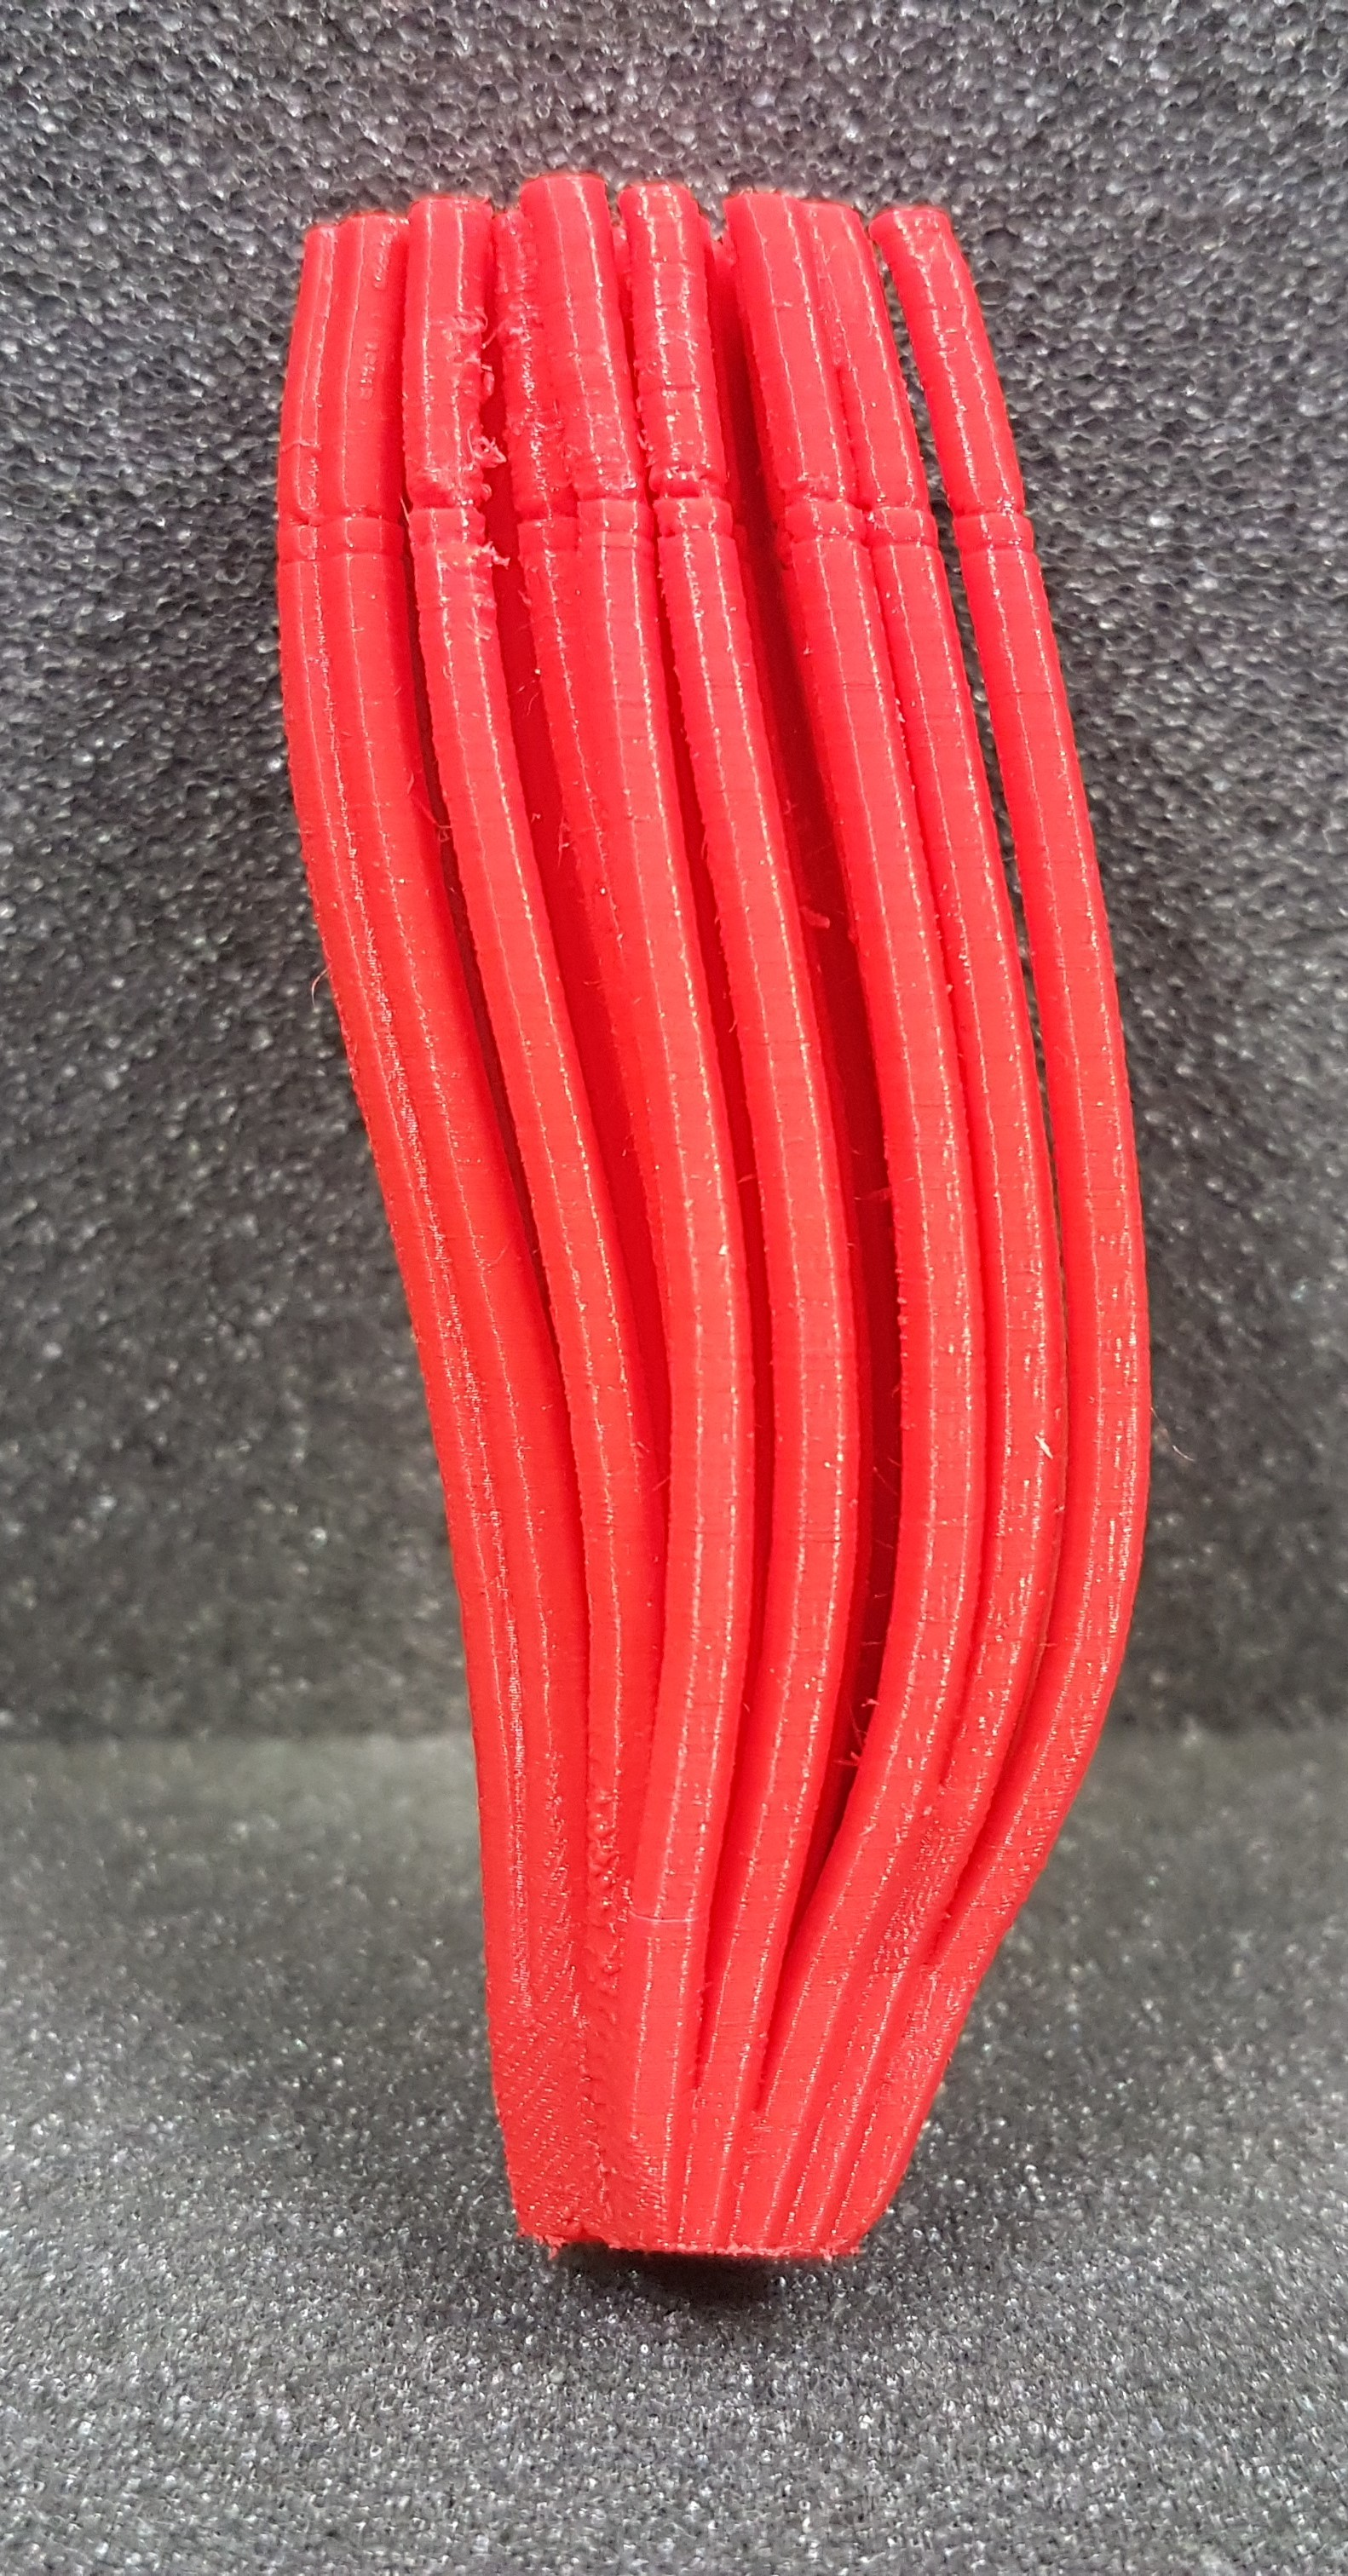
\includegraphics[width=.443\linewidth]{fascicles.jpg}
		\caption{A small, printed version of the biceps-model(left) and the fascicles (right)}
		\label{fig:printedBiceps}
\end{figure}

\section{Discussion}
%TODO Einleitung
During development and printing, we faced difficulties we had to work around. 
Therefore we made some observations and decisions, which we discuss here, including limitations of the material and software, and choosing certain values.

Reclassifying the Mesh is done by hand since Gmsh does not allow reclassifying a mesh by command line with parameters. 
For our Model it is critical to set the threshold to zero. 
This is because Gmsh would see the surface of the muscle as one, when a higher threshold was chosen.

When working with meshes the resolution plays a key role. 
The model we used was smooth but we noticed a significant increase in quality as we refined the mesh before executing the pipeline. 
Increasing the amount of nodes without a more detailed model can be accomplished by splitting the triangles in half.
We managed to refine the mesh up to two times, before Gmsh crashed.
This increases the number of tetrahedrons by the factor of four. 

When calculating in the refined setup, the streamlines pass a lot more edges of the tetrahedrons inside the muscle and as a consequence get a correction in terms of direction and force. 
As a result we receive smoother streamlines, which are distributed more evenly. 
This can be seen in figure ~\ref{fig:refStreamlines}.
The refined mesh results in the streamlines having more curvature and cover the volume more evenly.
The two lowest streamlines in the figures show this difference quite accurately.
While the unrefined mesh results in more edges and the two streamlines being too close to each other, the refined one is smoother and the fascicles position themselves closer to the surface.

When looking into runtime, the biggest factor is the number of points.
Refining the model increases the runtime significantly. 
The number of streamlines only plays a minor part when it is in a reasonable range.
We had no problem calculating over 10.000 streamlines. When trying to calculate 250.000 streamlines the runtime exceeds several minutes.

\begin{figure}
	\begin{minipage}{\linewidth}
		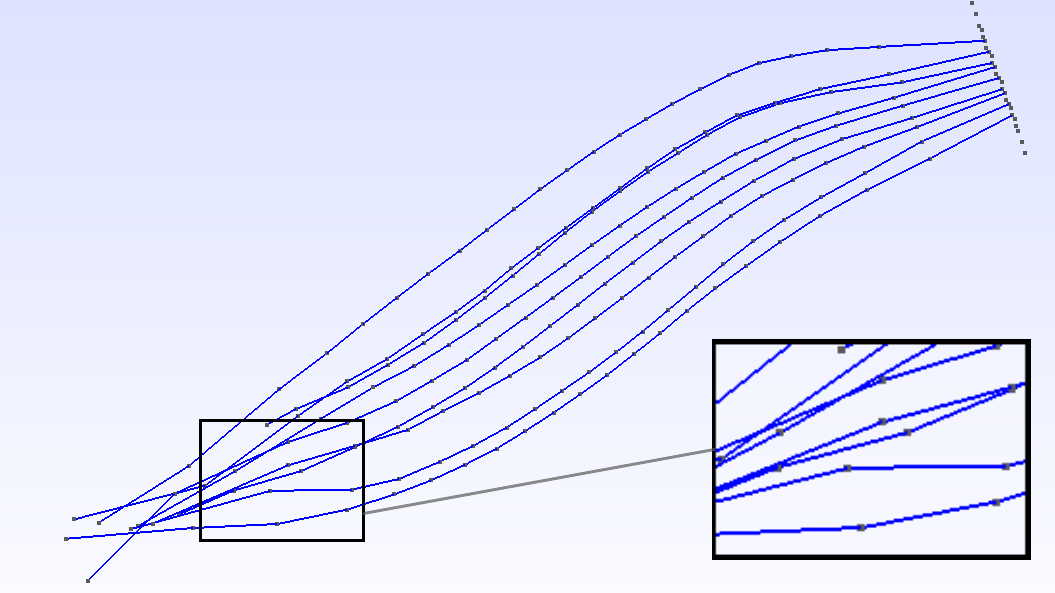
\includegraphics[width=.5\linewidth]{Streamlines_zoom.PNG}
		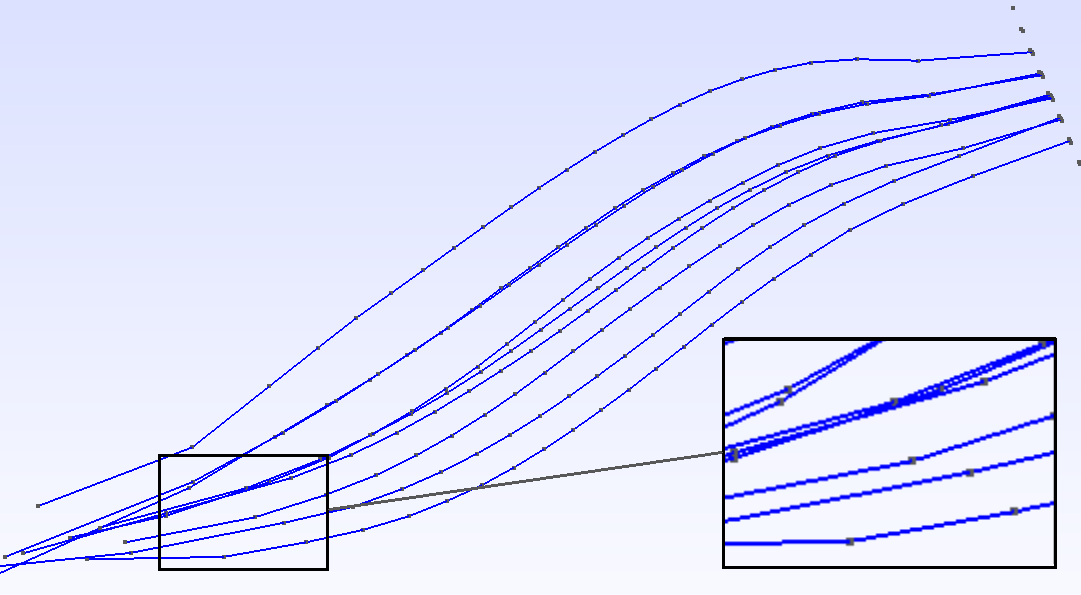
\includegraphics[width=.51\linewidth]{refStreamlines_zoom.PNG}
		\caption{Comparison of the two different mesh densities and the resulting resolution of the streamlines. In the right picture the mesh has been refined.}
		\label{fig:refStreamlines}
	\end{minipage}
\end{figure}

\section{Conclusion}
In conclusion we achieved our goal of developing a method for calculating muscular fascicles, based on the CT-scan.
We provide the possibility, to specify the amount of streamlines, and the number of mesh refinements. 
We applied the same procedure to a scan of the musculus triceps brachii as well. 
The result has a similar quality as the biceps.
Thus it is possible to try out further muscles and calculate their fascicle arrangement as well.
The plan was to print red streamlines into the transparent muscle with the help of the dual-printing function of the Ultimaker, but our two materials weren't compatible with each other. 

The resolution of the streamlines is currently limited to the resolution of the biceps CT-scan data. 
Therefore, in order to improve the quality of the streamlines e.g. edge-smoothing, a CT-scan with a higher resolution is needed. 
This way we can get an even better distribution of the fascicles.

\section{Future work}
The realistic fascicles promise improvement in biomechanical simulations, as one is able to contract the muscle along the fibers, resulting in more realistic modeling. 
Another possible work is to look into giving the calculated fascicles thickness based on measurements. 
The challenge would be to fit a reasonable amount of fibers inside of the model without exceeding the boundaries.
We have only scratched the surface of this topic in order to print the muscle.

We tried several approaches on printing but there are many more, which may result in better results.
It is also possible to model the muscle with it's fascicles using epoxy, but one must find a way to insert the the fibers into the muscle or rather create them beforehand and stabilize them while the epoxy of the muscle is hardening.
The advantage of this procedure would be, that the muscle can be transparent and an improvement regarding stability of the model.
%TODO mehr text, mehr dinge, mehr mehr (epoxyd-harz, andere herangehensweisen für printing)

\bibliographystyle{abbrv}
%%use following if all content of bibtex file should be shown
%\nocite{*}
\bibliography{documentation}
\end{document} 
